\documentclass[letterpaper,10pt]{article}

\usepackage{enumitem}
\usepackage{titling}
\usepackage{listings,listings-rust}
\usepackage{url}
\usepackage{soul}
\usepackage{hyperref}
\usepackage{setspace}
\usepackage{subfig}
\usepackage{sectsty}
\usepackage{pdfpages}
\usepackage{colortbl}
\usepackage{multirow}
\usepackage{multicol}
\usepackage{relsize}
\usepackage{amsmath}
\usepackage{wasysym}
\usepackage{fancyvrb}
\usepackage[yyyymmdd]{datetime}
\usepackage{amsmath,amssymb,amsthm,graphicx,xspace}
\usepackage[titlenotnumbered,noend,noline]{algorithm2e}
\usepackage[compact]{titlesec}
\usepackage{XCharter}
\usepackage[T1]{fontenc}
\usepackage[scaled]{beramono}
\usepackage[normalem]{ulem}
\usepackage{booktabs}
\usepackage{tikz}
\usetikzlibrary{arrows.meta,automata,shapes,trees,matrix,chains,scopes,positioning,calc,decorations.pathreplacing}
\tikzstyle{block} = [rectangle, draw, fill=blue!20, 
    text width=2.5em, text centered, rounded corners, minimum height=2em]
\tikzstyle{bw} = [rectangle, draw, fill=blue!20, 
    text width=4em, text centered, rounded corners, minimum height=2em]

\definecolor{namerow}{cmyk}{.40,.40,.40,.40}
\definecolor{namecol}{cmyk}{.40,.40,.40,.40}
\renewcommand{\dateseparator}{-}

\let\LaTeXtitle\title
\renewcommand{\title}[1]{\LaTeXtitle{\textsf{#1}}}

\lstset{basicstyle=\footnotesize\ttfamily,breaklines=true}

\newcommand{\CPP}{C\nolinebreak\hspace{-.05em}\raisebox{.4ex}{\tiny\bf +}\nolinebreak\hspace{-.10em}\raisebox{.4ex}{\tiny\bf +}}
\def\CPP{{C\nolinebreak[4]\hspace{-.05em}\raisebox{.4ex}{\tiny\bf ++}}}

\newcommand{\handout}[5]{
  \noindent
  \begin{center}
  \framebox{
    \vbox{
      \hbox to 5.78in { {\bf ECE459: Programming for Performance } \hfill #2 }
      \vspace{4mm}
      \hbox to 5.78in { {\Large \hfill #4  \hfill} }
      \vspace{2mm}
      \hbox to 5.78in { {\em #3 \hfill \today} }
    }
  }
  \end{center}
  \vspace*{4mm}
}

\newcommand{\lecture}[3]{\handout{#1}{#2}{#3}{Lecture#1}}
\newcommand{\tuple}[1]{\ensuremath{\left\langle #1 \right\rangle}\xspace}

\addtolength{\oddsidemargin}{-1.000in}
\addtolength{\evensidemargin}{-0.500in}
\addtolength{\textwidth}{2.0in}
\addtolength{\topmargin}{-1.000in}
\addtolength{\textheight}{1.75in}
\addtolength{\parskip}{\baselineskip}
\setlength{\parindent}{0in}
\renewcommand{\baselinestretch}{1.5}
\newcommand{\term}{Winter 2020}

\singlespace


\begin{document}

\lecture{ 35 --- Rust }{\term}{Patrick Lam \& Jeff Zarnett}

\section*{This, Too, Shall Fade and Pass Away}
In ECE~459 we've used C and \CPP~as systems languages. A lot of your previous courses have been in one of those and it's entirely possible that one of those was your first programming language and perhaps even the one you've used the most. The languages themselves have their strengths and weaknesses, of course, but there's no denying that these languages come without some of the niceties found in other languages like clever static type checking and garbage collection.


The nature of the languages make it hard, or even impossible, to write code that is fast, correct, and secure. The focus of this course hasn't been on security. But in many cases, writing insecure fast code isn't the right thing. Is it even possible to write secure C and \CPP?

Maybe not. The usual arguments are something along the lines of experience. Experience isn't it either, given this quotation from Robert O'Callahan: ``I cannot consistently write safe C/\CPP~ code.\footnote{\url{https://robert.ocallahan.org/2017/07/confession-of-cc-programmer.html}}'' (17 July 2017) (Holds a PhD in CS from Carnegie Mellon University; was Distinguished Engineer at Mozilla for 10 years; etc.)

What about use of better tools and best practices? March 2019: disclosure of Chrome use-after-free vulnerability\footnote{\url{https://security.googleblog.com/2019/03/disclosing-vulnerabilities-to-protect.html}}; 0-day attacks
observed in the wild. Google implements best practices, and has all the tools and developers that
money can buy!

Much of the advice about how to avoid these problems comes down to ``try harder'', which is... not helpful. If the strategy is just dragging people and saying that they need to pay more attention, or be more careful, or other similar phrase... this is going to constantly be an uphill battle. Expecting people to be perfect and make no mistakes is unrealistic. What we want is to make mistakes impossible.

A lot of the problems we frequently encounter are the kind that can be found by Valgrind, such as memory errors or race conditions. Other tools like code reviews and Coverity (static analysis defect-finding tool) exist. These are good, but not perfect. Valgrind, for example, only reports errors that it actually sees executed, so until and unless every function and every code path is run, it might not report a problem. Static analysis tools try to track down problems at compile-time, and that seems like a lot better of a solution.


I like to solve not just an individual problem, but an entire class of problems all at once. A recent example: if you change the contents of a list in a background thread while it's being rendered, the rendering thread will fail because the list has changed. I can fix the line of code so the list manipulation does not happen during rendering, and that fixes it once, but not forever: in the future another person could write code that calls this function from a background thread. There's no good way (in Java, sadly) to make it so invoking this function incorrectly is a compile-time error, so the best I can do is set a trap in it that throws an error if called inappropriately, so that the responsible developer will find what they did wrong during development and testing. Compile-time error checking is preferable to run-time.

This brings us to Rust. It is an alternative to C/\CPP. It is a new-school
secure systems programming language used by Mozilla's Project Quantum. A design goal of this language is to avoid issues with memory allocation and concurrency. We'll consider both concepts, but we won't dwell too much on the syntax (mostly for time reasons). It's worth reading up on the topic (outside of lecture) if you are curious about the language, though, and it might help you to understand the examples better.  

\section*{Rust} This material is based
on \emph{The Rust Programming Language} by Steve Klabnik and Carol
Nichols~\cite{klabnik18:_rust_progr_languag} and I'll make references as appropriate.

Here's some Rust code.
\vspace*{-.5em}
\begin{lstlisting}[language=Rust]
  fn main() {
    let x = 42; // NB: Rust infers type "s32" for x.
    println!("x is {}", x);
  }
\end{lstlisting}
By default, Rust variables are \emph{immutable}.
\vspace*{-.5em}
\begin{lstlisting}[language=Rust]
  fn main() {
    let x = 42; // NB: Rust infers type "s32" for x.
    x = 17; // compile-time error!
  }
\end{lstlisting}
Let's consider two examples that look similar but have drastically different meanings.

\vspace*{-1.5em}
\begin{minipage}{.4\textwidth}
\begin{lstlisting}[language=Rust]
  let x = 1729;
  let x = 88;
  println!("shadowed x is {}", x);
\end{lstlisting}
\end{minipage}\
\begin{minipage}{.4\textwidth}
\begin{lstlisting}[language=Rust]
  let mut x = 33; // mutable
  x = 5;
  println!("mutated x is {}", x);
\end{lstlisting}
\end{minipage}

In the first case, old ``x'' still exists but is inaccessible under the name ``x''.
In the second case, the storage cell for ``x'' used to contain 33 and then contains 5.
The difference matters, for instance, when there are references to ``x''. This example is a bit silly though; the real usage for shadowing is perhaps something more familiar, specifically parsing (or other transformation): 

\begin{lstlisting}[language=Rust]
let mut guess = String::new();

io::stdin().read_line(&mut guess)
    .expect("Failed to read line");

let guess: u32 = guess.trim().parse()
     .expect("Please type a number!");
\end{lstlisting}

In this example, the data is read in as a string and then turned into an unsigned integer. We like this because we can re-use the variable name without having things like \texttt{guess} and \texttt{guess\_parsed} or other ``what do I call this now'' problems.

\paragraph{Rust immutability.} 
By default, a variable in Rust is immutable. You can make it mutable if you choose, explicitly by declaring it as mutable. Lots of concurrency issues involve the internal state of objects that are accessed by different threads. Structs or tuples are either all mutable or all immutable.(Although interior mutability is a thing in Rust. We're not talking about it.)

Rust obviously has compile-time constants and they are truly unmodifiable. These have to be known at compile time, and are truly a fixed value. This is different from an immutable type which is determined at runtime but cannot be changed once it has been assigned.

In C, you can cast away {\tt const}-ness; not so in Rust.
If something is not mutable in Rust, you can't cast it into mutability.


\paragraph{Perf implications.}
We mentioned immutability in Lecture 7. The best way to avoid having
to use locks (even read/write locks still require writes to acquire
the read lock): have no writes.  However, there's a tradeoff. If your
data structure is immutable but you want to update it (as we often do
with data structures), you need to copy the data structure, at least
partially. That can be slow.


\paragraph{Runtime safety.} We said that Rust is safe. One way in which it is safe is for
arrays. Rust has tuples and structs. Hard to go out of bounds on those. Rust also has arrays.
Like with any language, one can imagine going beyond the ends of an array. Rust defines
the behaviour of going beyond the end of an array: it is a runtime exception (``panic''),
unlike C/\CPP, where it is undefined behaviour.


\begin{lstlisting}[language=Rust]
  let a = [1,2,3,4,5];
  let index = 10;
  println!("error! {}", a[index]); // panics here.
\end{lstlisting}

\subsection*{What's special about Rust?}
Let's step back and do some Rust propaganda.
\begin{itemize}[noitemsep]
\item harder to write unsafe code: compiler + runtime ensure safety. No arrays-out-of-bounds accesses, null pointers (at all), wild pointers;
\item yet can still write low-level code;
\item supports zero-cost abstractions (like \CPP);
\item designed with ergonomics in mind;
\item type system obviates need for either garbage collection or manual memory management (which you will get wrong)\footnote{Well, mostly. Sometimes you need to use ref-counted data, and we'll see that.};
\item type system prevents race conditions;
\item dependency management using crates.
\end{itemize}
As far as I know, Firefox's rendering engine, Project Servo, is the largest deployed Rust codebase. [size?]


\section*{Ownership in Rust [Chapter 4.1]}
Also known as ``how to fight the borrow checker and win''.

Rust uses ownership types to manage its heap. Ownership types were not invented by the Rust
community, but Rust is the first production-scale language to deploy it. The alternatives
are {\tt malloc}/{\tt free} in C, or {\tt new}/GC in Java. Rust does still have a stack, but
we'll see when things go on the stack vs when they go on the heap.

\subsection*{The Rules}
\begin{enumerate}[noitemsep]
\item Each value in Rust has a variable that \emph{owns} it.
\item This variable is \emph{unique}.
\item When the owner goes out of scope, the value will be dropped (aka freed).
\end{enumerate}

Variable scopes are fairly standard.
\begin{lstlisting}[language=Rust]
  fn main() {
    println!("start");
    { // no s
      let s = "I am s";
      println!("s is {}", s);
    } // s now out of scope
  }
\end{lstlisting}

OK, let's put something on the heap. We'll be using Rust {\tt String} objects rather than
string literals. String literals are compile-time constants. String objects contain a heap component,
which may be allocated and freed.

(What can go wrong with heap allocation? You might not free/free too late;
free too early; double free. GC manages this through an approximation: if you have no more pointers to it,
then it doesn't spark joy, and you don't need it anymore. Rust goes a different way.)
\begin{lstlisting}[language=Rust]
  fn main() {
    let s = String::from("hello"); // immutable String
    let mut s2 = String::from("459 assignments"); // mutable String
    s2.push_str(", maybe?");
    println!("got string {}", s);
  }
\end{lstlisting}

Rust uses rule \#3: if something goes out of scope, then drop (free) it.
This is quite like \CPP~RAII (Resource Acquisition is Initialization).

Still, we need a solution for objects that live beyond their original scope, e.g.
return values.
\begin{lstlisting}[language=Rust]
  fn return_a_string() -> String {
    let s = String::from("longevity");
    return s; // transfers ownership (moves) to caller
  }

  fn main() {
    let returned_string = return_a_string();
    println!("string {}", returned_string);
  }
\end{lstlisting}

So, Rust frees owned values when variables go out of scope. Also, Rust calls
``drop'' (akin to a destructor) on objects that go out of scope. Note that
going out of scope, not the drop call, is what actually causes the free.

\section*{Transferring Ownership (aka move semantics)}

Let's look at an example.
\begin{lstlisting}[language=Rust]
  let s1 = String::from("no surprise");
  println!("can print {}", s1);
  let s2 = s1;
  println!("can still print {}", s2);
  println!("this line won't compile! {}", s1); // no longer owns
\end{lstlisting}

(Note that string literals, or ints, or anything only on the stack,
doesn't have this behaviour---they are copied, or technically, they
have the ``Copy'' trait.)

OK, so what's going on? Let's take a step back.

Rust strings are a hybrid, containing both a stack part and a heap part.

\begin{center}
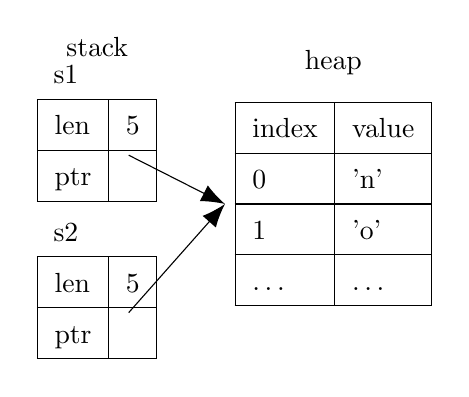
\begin{tikzpicture}
\draw (0,1) node {stack};
\draw (0,0) node (one) {
\begin{tabular}{|l|l|}
\multicolumn{2}{l}{s1} \\
\hline
len & 5 \\ \hline
ptr & \\ \hline
\end{tabular}
};

\draw (0,-2) node (two) {
\begin{tabular}{|l|l|} 
\multicolumn{2}{l}{s2} \\ \hline
len & 5 \\ \hline
ptr & \\ \hline
\end{tabular}
};

\draw (3,0.8) node {heap};
\draw (3, -1) node (s) {
\begin{tabular}{|l|l|} \hline
index & value \\ \hline
0 & 'n' \\ \hline
1 & 'o' \\ \hline
\ldots & \ldots \\ \hline
\end{tabular}
};

\path[draw,-{Latex[length=3mm]}] (one) ++ (0.4,-0.38) -- (s.west);
\path[draw,-{Latex[length=3mm]}] (two) ++ (0.4,-0.38) -- (s.west);

\end{tikzpicture}
\end{center}

The assignment {\tt let s2 = s1} carries out a shallow copy of the stack part. Rust
does not automatically copy the heap part.

Now, recall that Rust has automatic memory reclamation. How can that
work? What gets freed?  Here, {\tt s1} and {\tt s2} are in the same
scope. When they go out of scope, what should get freed? We
don't want to double free.

\paragraph{Key idea.} For automatic memory reclamation to work, we give {\tt let s2 = s1} \emph{move semantics}
(as in \CPP). After the move, {\tt s1} is no longer valid.
Ownership of the heap part is moved from {\tt s1} to {\tt s2} by the assignment.

That is, {\tt s1} no longer owns the heap object and is not responsible for freeing the heap part
when it goes out of scope. Only when {\tt s2} goes out of scope do we free the heap object.
And because the heap object only has one owner, it is only freed once.

Note: deep copy is possible with ``clone'', but we have to trigger that explicitly.

Want to know more about ownership? Here's a blog post:
\begin{center}
  \url{http://squidarth.com/rc/rust/2018/05/31/rust-borrowing-and-ownership.html}
\end{center}
\section*{Functions and Return Values}

Move semantics also applies to function calls and return values, e.g.
\begin{lstlisting}[language=Rust]
  fn main() {
    let s = String::from("moving to callee");
    callee(s); // afterwards, s is invalid
  }
  fn callee(param:String) {
    println!("got {}, param");
  } // param goes out of scope, object dropped
\end{lstlisting}
If you return something, then the ownership passes back to the caller.
Tuples help pass ownership of multiple objects, but this is still quite
high-overhead for developers.

\paragraph{``Can I please borrow your object?''}
\begin{lstlisting}[language=Rust]
  fn main() {
    let s = String::from("459");
    let len = calculate_length(s);
    println!("string {} has length {}", s /* we still have it! */,
             len);
  }
  fn calculate_length(s:&String) -> usize { // note the & for borrow
    s.len() // last expr is return value
  } // s is ref so nothing goes out of scope
\end{lstlisting}
  
\section*{Borrowing and mutation} Like other variables, references are immutable by default.
We can have mutable references, though.
\begin{lstlisting}[language=Rust]
  fn change(s:&mut String) {
    s.push_str("more");
  }
  fn main() {
    let mut main_str = String::from("some ");
    change(&mut main_str); // create mutable ref to main_str
  }
\end{lstlisting}

\paragraph{There can be only one (mutable).} The following code won't compile:
\begin{lstlisting}[language=Rust]
  let mut s = String::from("one");
  let r1 = &mut s;
  let r2 = &mut s; // rustc complains!
\end{lstlisting}
In fact, while {\tt r1} is in scope, you can't do anything with the original {\tt s}.
The only way to access the string is through {\tt r1}. Once {\tt r1} goes out of scope,
you can create {\tt r2}.

Since there is only one way to access {\tt r1}, then there will be no race conditions.

This is OK:
\begin{lstlisting}[language=Rust]
  let mut s = String::from("one");
  let r1 = &s;
  let r2 = &s; // no problem!
\end{lstlisting}
But you can't then do {\tt let r3 = \&mut s;}.

\paragraph{How many?} You can have as many outstanding immutable refs as you want.
If there are any immutable refs, you can't have \emph{any} mutable refs. The immutable
refs must go out of scope first.

You also can't commit use-after-free errors: you can't return a ref that outlives
its value.
\begin{lstlisting}[language=Rust]
  fn dangle() -> &String {
    let s = String::from("hello");
    &s // rustc complains: s goes out of scope with active refs
  }
\end{lstlisting}

Rust also has \emph{smart pointers}, which may be reference
counted. This is like \CPP's smart pointers, specifically {\tt
  shared\_ptr} (but Rust can tell you about some things at compile
time which \CPP~will tell you at runtime). Normal Rust objects are more
like {\tt unique\_ptr}.

We need reference counted heap objects e.g. to implement graphs. We don't have
enough time to talk about smart pointers, but Chapter 15 of the Rust book is good.

\section*{Fearless Concurrency}
As with many other aspects of Rust, we trade compiler errors for runtime
errors; in this case, runtime concurrency errors like race conditions.
That is, the type system ensures concurrency safety!

Rust uses a fork/join model like pthreads. It delegates to the operating
system's threads support and hence implements 1:1 threads.
\begin{lstlisting}[language=Rust]
  let handle = thread::spawn(|| { // closure (can put args between ||)
    // thread code goes here
  });
  // main thread continues here
  handle.join.unwrap(); // unwrap: panic in case of error
\end{lstlisting}
This is not too different from \CPP.

OK, how do we share data between threads? We can move it from main to thread:
\begin{lstlisting}[language=Rust]
  let v = vec![1,2,3];
  let handle = thread::spawn(move || { // move: everything accessed inside closure is moved
    println!("vector {:?}", v);
  }); // no longer have access to v in main
  handle.join().unwrap();
\end{lstlisting}
Rust is saving you from being able to concurrently access {\tt v} in main and thread.

But that's only one way! This isn't quite enough.

\subsection*{Message Passing}
One way to share data is message passing. We've seen this before (OpenMPI).
In this case, each value still only has one owner. We use \emph{channels}. The ownership passes
from the sender, through the channel, to the receiver.
\begin{lstlisting}[language=Rust]
  use std::thread;
  use std::sync::mpsc; // multi producer, single consumer

  fn main() {
    let (tx, rx) = mpsc::channel(); // tx is cloneable
    thread::spawn(move || { // here, tx goes to closure
      let val = String::from("april");
      tx.send(val).unwrap(); // val moved from sender
    });
    let received = rx.recv().unwrap();
    println!("got: {}", received);
  }
\end{lstlisting}
Note the send/receive pair. There is also {\tt try\_recv} to do nonblocking receives.

\subsection*{Shared State}
People debated for a long time which was better: shared state (like pthreads) or channels.
Rust supports both. Of course, the problem with shared state is race conditions.
Like manual memory management, we can manually acquire and release mutexes. What could
possibly go wrong? Rust's ownership system will help.

We'll need to talk about multiple ownership. But let's talk about mutexes first.
\begin{lstlisting}[language=Rust]
  use std::sync::Mutex;
  fn main() {
    let m = Mutex::new(5); // mutex guards access to an i32
    {
      let mut num = m.lock().unwrap();
      // unwrap: maybe some other thread panicked while holding lock;
      //         then we panic too.
      *num = 6; // "deref" the mutex (is actually a smart pointer)
    } // release lock when num goes out of scope
    println!("m={:?}", m);
  }
\end{lstlisting}
Well, that's fine, but it's just one thread. We really do need multiple ownership
to share data. The shared data needs to be owned by all threads, and a naive solution
will get rejected by the borrow checker. Instead, we have to use \emph{reference counted
  cells}, implemented by {\tt Arc}.
% end of 3rd lecture
\begin{lstlisting}[language=Rust]
  use std::sync::{Mutex, Arc};
  use std::thread;
  fn main() {
    let counter = Arc::new(Mutex::new(0)); // atomic reference cell
    let mut handles = vec![];

    for _ in 0..10 {
      let counter = Arc::clone(&counter); // clone the Arc
      let handle = thread::spawn(move || {
        let mut num = counter.lock().unwrap();
        *num += 1;
      });
      handles.push(handle);
    }
    for handle in handles {
      handle.join().unwrap();
    }
    println!("result: {}", *counter.lock().unwrap());
  }
\end{lstlisting}
Rust guarantees that you have the appropriate lock, using ownership (possibly multiple ownership).
Rust does not guarantee lack of deadlocks.


\bibliographystyle{alphaurl}
\bibliography{459}


\end{document}
